\documentclass[12pt]{article}

\usepackage[paper=letterpaper, margin=0.5in, footskip=0.25in]{geometry}
% margins can easily be changed in the line above;
% footskip sets the position of page numbers
\usepackage{amsmath}                % for math enhancements
\usepackage{datetime}               % for custom date/time format
\usepackage{amssymb}                % for extra math symbols
\usepackage{titlesec}               % for custom title/section/subsection formats
\usepackage{enumitem}               % for numbered lists
\usepackage{graphicx}               % for including images and other graphics
\usepackage{hyperref}               % for hyperlinks
\usepackage[skip=0.15em]{caption}   % for figure captions
\usepackage[font=normal]{subfig}    % for figures and subfigures
\usepackage{xcolor}                 % for coloring and highlighting text
\usepackage{pgfplots}               % for slope fields
\usetikzlibrary{calc}               % for slope fields
\pgfplotsset{compat=1.18}           % for slope fields
\usepackage{setspace}               % for 1.25 spacing
\usepackage{chngcntr}               % for managing equation numbering
\usepackage{bm}
\usetikzlibrary{shapes.arrows}

\counterwithin*{equation}{subsection}

\hypersetup{
	colorlinks   = true,    % colored links instead of boxes
	urlcolor     = blue,    % color for external hyperlinks
	linkcolor    = blue,    % color for internal links
	citecolor    = red      % color for citations
}

\newdateformat{monthyeardate}{\monthname[\THEMONTH] \THEYEAR}
% the line above sets the month and year automatically
% if you don't like this format, you can easily change it

\makeatletter
\def\@maketitle{
	\newpage
	\vspace*{-\topskip}
	\begingroup\centering
	\let \footnote \thanks
	\hrule height \z@
	{\fontsize{16}{19.2} \@title \par}
	\vskip 0.25em 
	{\large
		\lineskip 0.5em 
		\begin{tabular}[t]{c}
			\@author
		\end{tabular}\par}
	\vskip 0.25em 
	{\large \monthyeardate\today}
	\par\endgroup
	\vskip 1em
}
\makeatother

\titleformat{\section}{\normalfont\scshape}{\textbf\thesection}{0em{\textbf{ – }}}{\textbf \color{magenta}}
\titleformat{\subsection}{\normalfont\scshape}{\textit\thesubsection}{0em{\textit{ – }}}{\textit}
% if you don't like the italicized subsections, change all the textit commands
% in the line above to textbf or whatever else you prefer
\titlespacing*{\section}{0pt}{1.5em}{0.5em}
\titlespacing*{\subsection}{0pt}{1em}{0.33em}

\title{\textbf{Differential Equations Notes}}
\author{Erk Sampat}
\begin{document}
\maketitle

\begin{center}
	MATH 4B \\
	UC Santa Barbara \\
\end{center}
\setstretch{1.25}

\section{Tools for Differential Equations}
\subsection{Direction Fields}
The graph below is a \textbf{direction field} (or \textbf{slope field}) of the differential equation $\frac{dy}{dx} = x + y$. The magenta-colored lines represent a set of \textbf{integral curves} (or \textbf{solution curves}).

Each blue arrow represents the slope, $\frac{dy}{dx}$, at its tail. In other words, the slope attained when plugging the point of the tail into the differential equation. This is useful because it showcases the behavior of the differential equation across a wide range of $x$ and $y$ values.

The integral curves represent specific solutions to the differential equation. In this case, the general solution is $y = -x - 1 + ce^x$, where $c$ is a constant. Several solutions have been plotted, each with a different value of $c$. Note that the integral curves always flow tangent to the slope arrows.

\begin{center}
	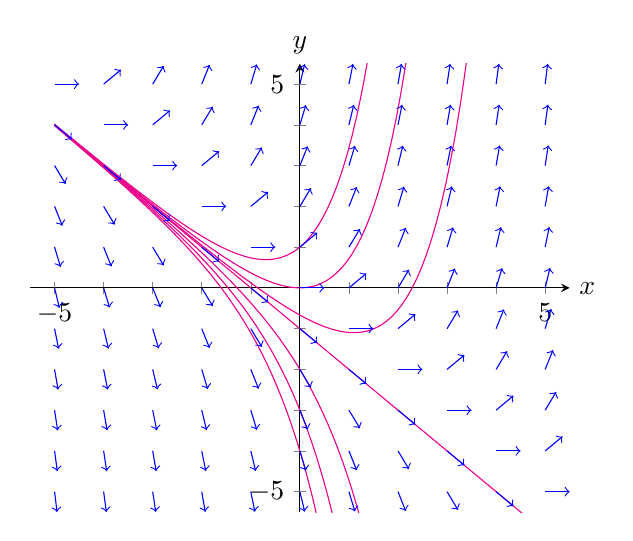
\begin{tikzpicture}
		\def\xmin{-5} \def\xmax{5}
		\def\ymin{-5} \def\ymax{5}
		\begin{axis}[
			axis x line=center,
			axis y line=center,
			xtick={\xmin,\xmin+1,...,\xmax},
			xticklabels={},
			extra x ticks={\xmin,\xmax},
			ytick={\ymin,\ymin+1,...,\ymax},
			yticklabels={},
			extra y ticks={\ymin,\ymax},
			xlabel={$x$},
			ylabel={$y$},
			xlabel style={right},
			ylabel style={above},
			xmin=\xmin-0.5,
			xmax=\xmax+0.5,
			ymin=\ymin-0.5,
			ymax=\ymax+0.5]
			\addplot[color=magenta,samples=100]{-x - 1 + (e^x)/3}; % y = -x - 1 + ce^x
			\addplot[color=magenta,samples=100]{-x - 1 + e^x};
			\addplot[color=magenta,samples=100]{-x - 1 + 2*e^x};
			\addplot[color=magenta,samples=100]{-x - 1};
			\addplot[color=magenta,samples=100]{-x - 1 - e^x};
			\addplot[color=magenta,samples=100]{-x - 1 - 2*e^x};
			\addplot[color=magenta,samples=100]{-x - 1 - 3*e^x};
			\foreach \n in {\ymin,...,\ymax}
			\addplot[blue,quiver={u={1/sqrt(1+(x+y)^2)},v={(x+y)/sqrt(1+(x+y)^2)},scale arrows=0.5},->,samples=2*\xmax + 1,]{\n};
		\end{axis}
	\end{tikzpicture}
\end{center}

\subsection{Integration by Parts}
If you have to integrate the product of an algebraic and a transcendental function like $xe^{x}$, you will probably need to integrate by parts. \textit{Choose the algebraic function for $u$, and the transcendental function for $v$.} Here's the formula:
$$\int uvdx = u\int vdx - \int \left(u'\int vdx\right)dx$$

Let's do a quick example. Integrate:
$$\int xe^{x}dx$$

\textit{Solution:}
$$u = x,\;v = e^{x}$$
$$\int xe^{x}dx = x\int e^{x}dx - \int \left(1\int e^{x}dx\right)dx$$
$$= xe^{x} - \int (e^{x})dx$$
\begin{center}
	= \boxed{xe^{x} - e^{x} + c}
\end{center}

\section{First-Order Differential Equations}
\subsection{Linear Equations}
In this section we are going to solve differential equations of the form: $$\frac{dy}{dt} + p(t)y(t) = g(t)$$

Let's start by multiplying everything by a function $u(t)$, called the \textbf{integrating factor}: $$u(t)\frac{dy}{dt} + u(t)p(t)y(t) = u(t)g(t)$$

We'll change $\frac{dy}{dt}$ to $y'(t)$, and we'll assume that $u(t)p(t)=u'(t)$: $$y'(t)u(t) + u'(t)y(t) = u(t)g(t)$$

On the left side, we merely have the product rule in action. We can thus rewrite the equation: $$(y(t)u(t))' = u(t)g(t)$$

Let's integrate:
$$\int (y(t)u(t))'dt = \int u(t)g(t)dt$$
$$y(t)u(t) = \int u(t)g(t)dt + c$$
$$y(t) = \frac{\int u(t)g(t)dt + c}{u(t)}$$

We now have a formula for $y(t)$. However, we still need to find the integrating factor $u(t)$. Remember: $$u(t)p(t)=u'(t)$$

Let's divide both sides by $u(t)$: $$p(t) = \frac{u'(t)}{u(t)}$$

Though it may be a little hard to recognize, the right side is equal to a simple derivative:
$$\frac{d}{dt}ln(u(t)) = \frac{1}{u(t)}u'(t)$$

We then have: $$ln(u(t))' = p(t)$$

Integrating and simplifying:
$$\int ln(u(t))'dt = \int p(t)dt$$
$$ln(u(t)) = \int p(t)dt$$
$$u(t) = e^{\int p(t)dt}$$

This is important. Let's say that $\int p(t)dt = q(t) + c$. Here's how we need to handle the $c$:
$$u(t) = e^{q(t) + c} = e^{q(t)}e^{c} = ce^{q(t)}$$

Believe it or not, we are ready to tackle an example problem. Solve the following IVP:
$$ty' + 2y = t^2 - t + 1,\;y(1) = \frac{1}{2}$$

\textit{Solution:}
$$y' + \frac{2}{t}y = t - 1 + \frac{1}{t}$$
$$u(t) = e^{\int \frac{2}{t}dt} = e^{2\int \frac{1}{t}dt} = e^{2ln(t)} = {e^{ln(t)}}^2 = t^{2}$$
$$t^{2}y' + 2ty = t^{3} - t^{2} + t$$
$$\int (yt^{2})'dt = \int (t^{3} - t^{2} + t)dt$$
$$yt^{2} = \frac{1}{4}t^{4} - \frac{1}{3}t^{3} + \frac{1}{2}t^{2} + c$$
$$y = \frac{1}{4}t^{2} - \frac{1}{3}t + \frac{1}{2} + \frac{c}{t^{2}}$$
$$\left(\frac{1}{2}\right) = \frac{1}{4}(1)^{2} - \frac{1}{3}(1) + \frac{1}{2} + \frac{c}{(1)^{2}}$$
$$\frac{1}{2} = \frac{1}{4} - \frac{1}{3} + \frac{1}{2} + c$$
$$c = \frac{1}{12}$$
\begin{center}
	\boxed{y(t) = \frac{1}{4}t^{2} - \frac{1}{3}t + \frac{1}{2} + \frac{1}{12t^{2}}}
\end{center}

\pagebreak

\subsection{Separable Equations}
We are now going to look at equations of the form:
$$N(y)\frac{dy}{dx} = M(x)$$

Let's start by integrating both sides with respect to $x$:
$$\int N(y)\frac{dy}{dx}dx = \int M(x)dx$$

$y = y(x)$, so let's use a change of variable and then integrate:
$$u = y(x),\;du = \frac{dy}{dx}dx = dy$$
$$\int N(u)du = \int M(x)dx$$

The above process is the mathematically correct way of solving the equation, but we can simply write:
$$\int N(y)dy = \int M(x)dx$$

Time for an example. Solve the following IVP and determine the interval of validity for the solution:
$$y' = e^{-y}(2x - 4),\;y(5) = 0$$

\textit{Solution:}
$$\frac{1}{e^{-y}}\frac{dy}{dx} = 2x - 4$$
$$\int e^{y}dy = \int (2x - 4)dx$$
$$e^{y} = x^{2} - 4x + c$$
$$y = ln(x^{2} - 4x + c)$$
$$(0) = ln((5)^{2} - 4(5) + c)$$
$$25 - 20 + c = 1$$
$$c = -4$$
\begin{center}
	\boxed{y(x) = ln(x^{2} - 4x - 4)}
\end{center}

\pagebreak

Here's what that quadratic $x^{2} - 4x - 4$ looks like. The roots are $2 \pm 2\sqrt{2}$:
\begin{center}
	\begin{tikzpicture}
		\def\xmin{-2} \def\xmax{6}
		\def\ymin{-10} \def\ymax{10}
		\begin{axis}[
			axis x line=center,
			axis y line=center,
			xtick={\xmin,\xmin+1,...,\xmax},
			xticklabels={},
			extra x ticks={\xmin,\xmax},
			ytick={\ymin,\ymin+1,...,\ymax},
			yticklabels={},
			extra y ticks={\ymin,\ymax},
			xlabel={$x$},
			ylabel={$y$},
			xlabel style={right},
			ylabel style={above},
			xmin=\xmin-0.5,
			xmax=\xmax+0.5,
			ymin=\ymin-0.5,
			ymax=\ymax+0.5]
			\addplot[color=magenta,samples=100,domain=\xmin:\xmax]{x^2 - 4*x - 4};
		\end{axis}
	\end{tikzpicture}
\end{center}

We can't take the natural log of 0 or a negative number. So the possible intervals of validity are $x = (-\infty, 2 - 2\sqrt{2})$ or $x = (2 + 2\sqrt{2}, \infty)$. We need to select the interval that contains our initial condition, so in this case, just \boxed{x = (2 + 2\sqrt{2}, \infty)}.

\subsection{Bernoulli Equations}
This is a fun section. We are going to solve equations of the form:
$$y' + p(x)y = q(x)y^{n}$$

We'll start by dividing the equation by $y^{n}$, which gives us:
\begin{equation}
	y^{-n}y' + p(x)y^{1 - n} = q(x)
\end{equation}

Let's use a substitution:
$$v(x) = y^{1 - n},\;v'(x) = (1 - n)y^{-n}y'$$

Here's how we obtained $v'$ above:
$$v' = \frac{dv}{dx} = \frac{dv}{dy}\frac{dy}{dx}$$
$$\frac{dv}{dy} = (1 - n)y^{-n},\;\frac{dy}{dx} = y'$$

Let's put our substitution to use, plugging it into (1):
$$\frac{v'}{1 - n} + p(x)v = q(x)$$

We now have a linear differential equation, and after solving for $v$, we can plug it back into our substitution to solve for $y$.

\pagebreak

Let's try an example. Solve the following IVP:
$$6y' - 2y = xy^{4},\;y(0) = -2$$

\textit{Solution:}
$$6y^{-4}y' - 2y^{-3} = x$$
$$v = y^{-3},\;v' = -3y^{-4}y'$$
$$-2v' - 2v = x$$
$$v' + v = -\frac{1}{2}x$$
$$u(x) = e^{\int dx} = e^{x}$$
$$e^{x}v' + ve^{x} = -\frac{1}{2}xe^{x}$$
$$\int (ve^{x})'dx = -\frac{1}{2}\int xe^{x}dx$$
$$ve^{x} = -\frac{1}{2}(xe^{x} - e^{x}) + c$$
$$v = -\frac{1}{2}(x - 1) + ce^{-x} = y^{-3}$$
$$y = \left(-\frac{1}{2}(x - 1) + ce^{-x}\right)^{-\frac{1}{3}}$$
$$-2 = \left(-\frac{1}{2}((0) - 1) + ce^{(0)}\right)^{-\frac{1}{3}}$$
$$-\frac{1}{8} = \frac{1}{2} + c$$
$$c = -\frac{5}{8}$$
\begin{center}
	\boxed{y(x) = \left(-\frac{1}{2}(x - 1) - \frac{5}{8}e^{-x}\right)^{-\frac{1}{3}}}
\end{center}

\subsection{Substitutions, Part 1}
We just learned about Bernoulli equations, where we used a substitution to convert the equation into something we could more easily solve. We are going to look at two more substitutions. The first one is for equations in the form:
\begin{equation}
	y' = F\left(\frac{y}{x}\right)
\end{equation}

We'll use the substitution:
\begin{equation}
	v(x) = \frac{y}{x}
\end{equation}

Rewriting it:
$$y(x) = xv(x)$$

Using the product rule, we find the derivative of $y$ with respect to $x$:
$$\frac{dy}{dx} = x'v(x) + xv'(x)$$

We'll change $\frac{dy}{dx}$ to $y'$, and we'll simplify the right side:
\begin{equation}
	y' = v + xv'
\end{equation}

Let's now plug our substitution into the original equation. (2) goes on the right side of (1), and (3) goes on the left side of (1):
$$v + xv' = F(v)$$

Though it may be hard to tell, we have separable equation. Let's solve it:
$$x\frac{dv}{dx} = F(v) - v$$
$$\int \frac{1}{F(v) - v}dv = \int \frac{1}{x}dx$$

It is best to learn the rest of the process through an example. Solve the following IVP:
$$xy' = y(ln(y) - ln(x)),\;y(1) = 4,\;x > 0$$

\textit{Solution:}
$$y' = \frac{y}{x}ln\left(\frac{y}{x}\right)$$
$$v = \frac{y}{x}$$
$$y = xv,\;y' = v + xv'$$
$$v + xv' = vln(v)$$
$$x\frac{dv}{dx} = vln(v) - v$$
$$\int \frac{1}{x}dx = \int \frac{1}{v(ln(v) - 1)}dv$$
$$u = ln(v) - 1,\;du = \frac{1}{v}$$
$$ln(x) = \int \frac{1}{u}du = ln(u) + c$$
$$ln(x) = ln(ln(v) - 1) + c$$
$$x = c(ln(v) - 1)$$
$$x = c\left(ln\left(\frac{y}{x}\right) - 1\right)$$
$$cx + 1 = ln\left(\frac{y}{x}\right)$$
$$\frac{y}{x} = e^{cx + 1} = ee^{cx} = ee^{c^{x}} = ec^{x}$$
$$y = xec^{x}$$
$$(4) = (1)ec^{1}$$
$$c = \frac{4}{e}$$
\begin{center}
	\boxed{y(x) = xe\left(\frac{4}{e}\right)^{x}}
\end{center}

\subsection{Substitutions, Part 2}
This is the last substitution we will learn. We'll solve equations of the form:
$$y' = G(ax + by)$$

We will use the substitution:
$$v = ax + by,\;v' = a + by'$$

Rewriting $v'$:
$$y' = \frac{v' - a}{b}$$

We'll plug this into the original equation and simplify things:
$$\frac{v' - a}{b} = G(v)$$
$$v' = bG(v) + a$$

Like we did in the last section, we have arrived at a separable differential equation:
$$\frac{dv}{dx} = bG(v) + a$$
$$\int dx = \int \frac{1}{bG(v) + a}dv$$

Let's do an example. Solve the following IVP:
$$y' - (4x - y + 1)^{2} = 0,\;y(0) = 2$$

\textit{Solution:}
$$y = (4x - y + 1)^{2}$$
$$v = 4x - y + 1,\;v' = 4 - y'$$
$$y' = 4 - v'$$
$$4 - v' = v^{2}$$
$$v' = \frac{dv}{dx} = 4 - v^{2}$$
$$\int dx = \int \frac{1}{4 - v^{2}}dv$$

We need to do a partial fraction decomposition:
$$\frac{1}{4 - v^{2}} = \frac{a}{2 + v} + \frac{b}{2 - v} = \frac{a}{2 + v}\cdot\frac{2 - v}{2 - v} + \frac{b}{2 - v}\cdot\frac{2 + v}{2 + v}$$
$$2a - av + 2b + bv = 1$$
$$bv - av = 0,\;2a + 2b = 1$$
$$a = b$$
$$2a + 2(a) = 1$$
$$a = b = \frac{1}{4}$$
$$\frac{1}{4 - v^{2}} = \frac{1}{8 + 4v} + \frac{1}{8 - 4v}$$

Resuming our original problem:
$$x = \int \frac{1}{8 + 4v}dv + \int \frac{1}{8 - 4v}dv$$
$$u = 8 + 4v,\;du = 4;\;w = 8 - 4v,\;dw = -4$$
$$x = \frac{1}{4}\int \frac{1}{u}du - \frac{1}{4}\int \frac{1}{w}dw$$
$$4x = ln(u) - ln(w) + c = ln\left(\frac{u}{w}\right) + c$$
$$e^{4x} = e^{ln(\frac{u}{w}) + c} = e^{c}e^{ln(\frac{u}{w})} = ce^{ln(\frac{u}{w})} = c\frac{u}{w}$$
$$e^{4x} = c\frac{8 + 4v}{8 - 4v} = c\frac{8 + 4(4x - y + 1)}{8 - 4(4x - y + 1)}$$
$$ce^{4x} = \frac{8 + 4(4x - y + 1)}{8 - 4(4x - y + 1)}$$
$$8ce^{4x} - 4ce^{4x}(4x - y + 1) = 8 + 4(4x - y + 1)$$
$$8ce^{4x} - 16cxe^{4x} + 4yce^{4x} - 4ce^{4x}= 8 + 16x - 4y + 4$$
$$4yce^{4x} + 4y = -4ce^{4x} + 16cxe^{4x} + 16x + 12$$
$$y(4ce^{4x} + 4) = -4ce^{4x} + 16cxe^{4x} + 16x + 12$$
$$y = \frac{-4ce^{4x} + 16cxe^{4x} + 16x + 12}{4ce^{4x} + 4}$$
$$y = \frac{-ce^{4x} + 4cxe^{4x} + 4x + 3}{ce^{4x} + 1}$$
$$2 = \frac{-ce^{4(0)} + 4c(0)e^{4(0)} + 4(0) + 3}{ce^{4(0)} + 1}$$
$$c = \frac{1}{3}$$
\begin{center}
	\boxed{y(x) = \frac{-\frac{1}{3}e^{4x} + \frac{4}{3}xe^{4x} + 4x + 3}{\frac{1}{3}e^{4x} + 1}}
\end{center}

\subsection{Equilibrium Solutions}
Let's look at the slope field of $y' = (y^{2} - 1.21)(y + 1)^{2}$ below:
\begin{center}
	\begin{tikzpicture}[scale=1.625]
		\def\xmin{-2} \def\xmax{2}
		\def\ymin{-2} \def\ymax{2}
		\begin{axis}[
			axis x line=center,
			axis y line=center,
			xtick={\xmin,\xmin+1,...,\xmax},
			xticklabels={},
			extra x ticks={\xmin,\xmax},
			ytick={\ymin,\ymin+1,...,\ymax},
			yticklabels={},
			extra y ticks={\ymin,\ymax},
			xlabel={$x$},
			ylabel={$y$},
			xlabel style={right},
			ylabel style={above},
			xmin=\xmin-0.5,
			xmax=\xmax+0.5,
			ymin=\ymin-0.5,
			ymax=\ymax+0.5]
			\addplot[color=magenta,samples=100]{-x - 1 + (e^x)/3}; % y = -x - 1 + ce^x
			\addplot[color=magenta,samples=100]{-x - 1 + e^x};
			\addplot[color=magenta,samples=100]{-x - 1 + 2*e^x};
			\addplot[color=magenta,samples=100]{-x - 1};
			\addplot[color=magenta,samples=100]{-x - 1 - e^x};
			\addplot[color=magenta,samples=100]{-x - 1 - 2*e^x};
			\addplot[color=magenta,samples=100]{-x - 1 - 3*e^x};
			\foreach \n in {\ymin,...,\ymax}
			\addplot[blue,quiver={u={1/sqrt(1+(x+y)^2)},v={(x+y)/sqrt(1+(x+y)^2)},scale arrows=0.5},->,samples=2*\xmax + 1,]{\n};
		\end{axis}
	\end{tikzpicture}
\end{center}

Notice that the slope is zero at $y = 3$ and $y = -2$.

\begin{center}
	\begin{tikzpicture}
		\def\xmin{-5} \def\xmax{5}
		\def\ymin{0} \def\ymax{0}
		\begin{axis}[
			axis x line=center,
			axis y line=none,
			xtick={\xmin,\xmin+1,...,\xmax},
			xticklabels={},
			extra x ticks={\xmin,\xmax},
			xlabel={$x$},
			xlabel style={right},
			xmin=\xmin-0.5,
			xmax=\xmax+0.5,
			ymin=\ymin-0.5,
			ymax=\ymax+0.5]
		\end{axis}
	\end{tikzpicture}
\end{center}
\end{document}